\chapter{活動}
\section{ブレインストーミング}
各々が開発したいアイデアを,Miro\footnote{https://miro.com/}を使用して,書き出した.
アイデアの例は以下である.

\begin{quote}
    \begin{itemize}
        \item 独り言を自動的に録音してテキスト化
        \item 健康促進アプリ(地図上でこれまで行った場所を塗りつぶす)
        \item 悩みがある人同士で会話できるもの
        \item 店など様々な場所の混雑度チェックアプリ
        \item 公共交通機関を携帯からリアルタイムに把握する
        \item 1日を可視化
    \end{itemize}
\end{quote}

各々違う色の付箋を使用し,KJ法を使用し意見をまとめた.
この活動ではさまざまな意見が挙げられたが,一番チームの共感を得たバス利用に関する問題について,今後の活動を絞った.

\begin{figure}[H]
    \centering
    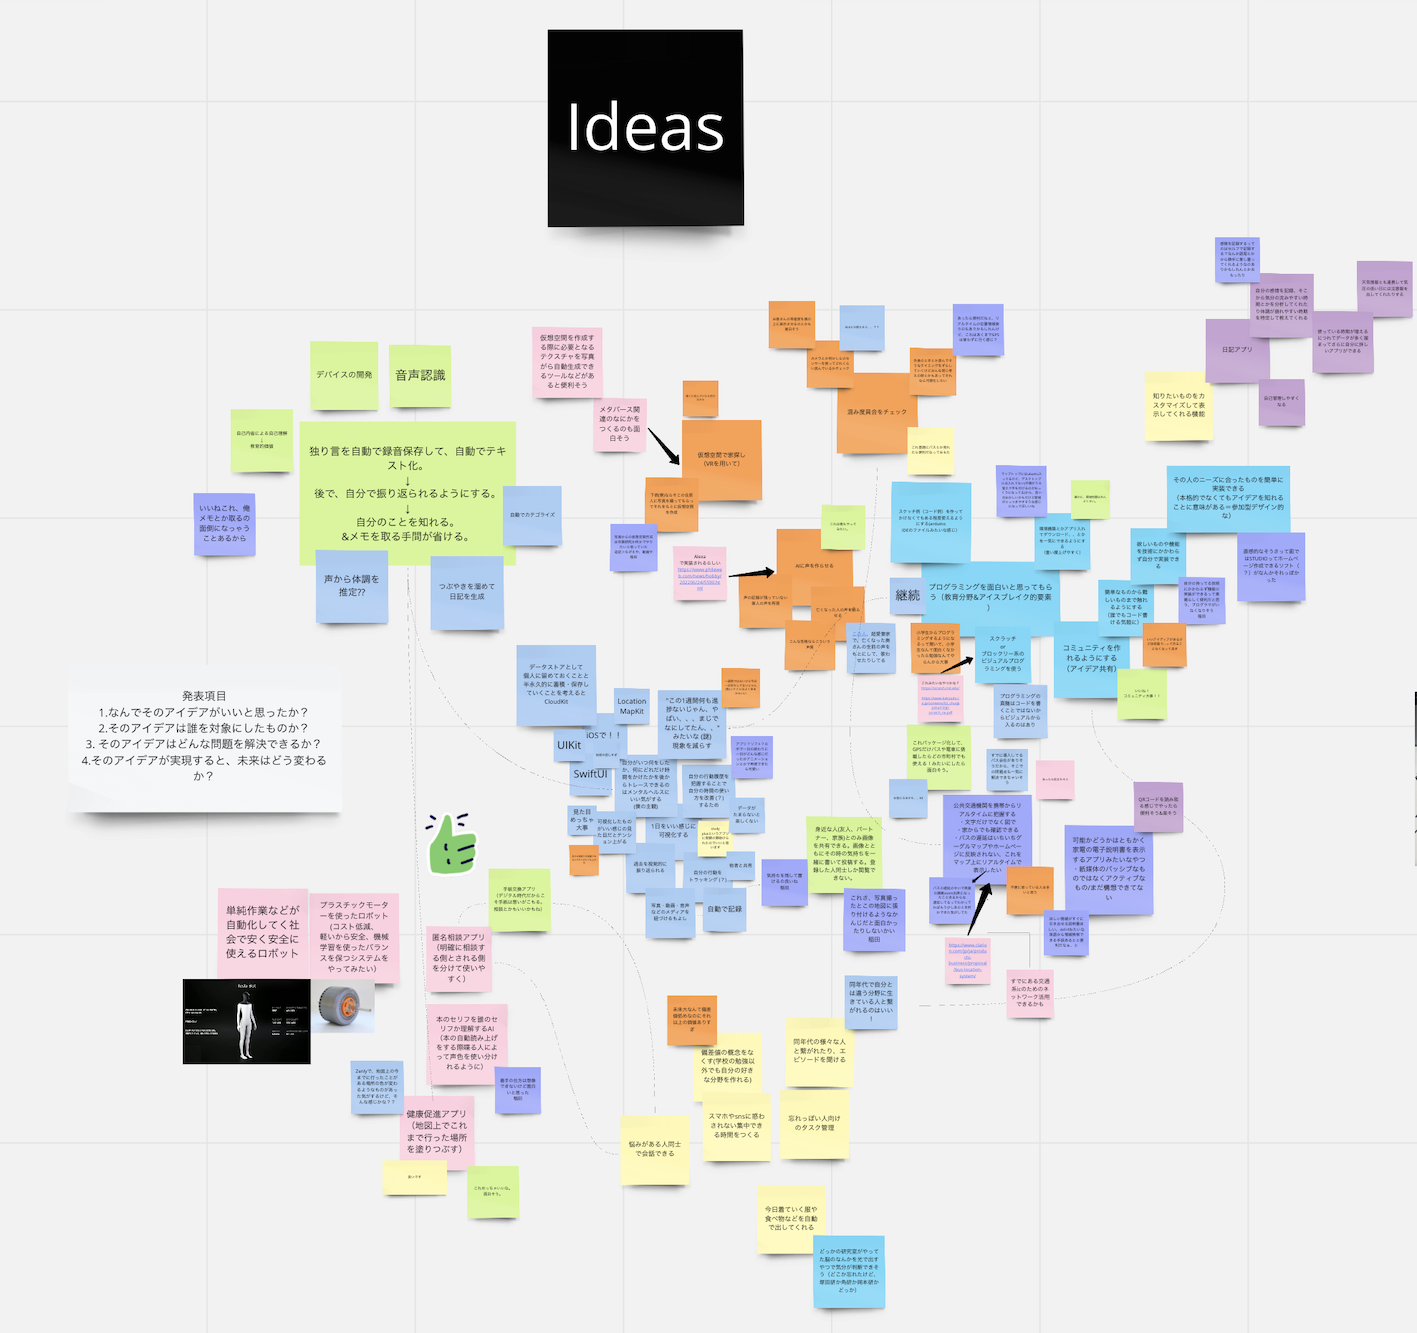
\includegraphics[width=9cm]{images/brainstorm.png}
    \caption{ブレインストーミング}
    \label{fig:brainstorm}
\end{figure}
\bunseki{大津武琉}

\section{アイデアの深掘り}

上記のブレインストーミングで挙げられたアイディアは煩雑なものであったため,実際に我々がバスを利用してきた中で不便に感じたことを考え,
解決策への仮説を列挙した.以下はその例である.

\begin{quote}
    \begin{itemize}
        \item 交通系ICカードを取り込み残高を表示
        \item バス停までの徒歩時間表示
        \item バスの時刻表表示
        \item 地図上に表示するバスの数を変えることができる
    \end{itemize}
\end{quote}

\begin{figure}[H]
    \centering
    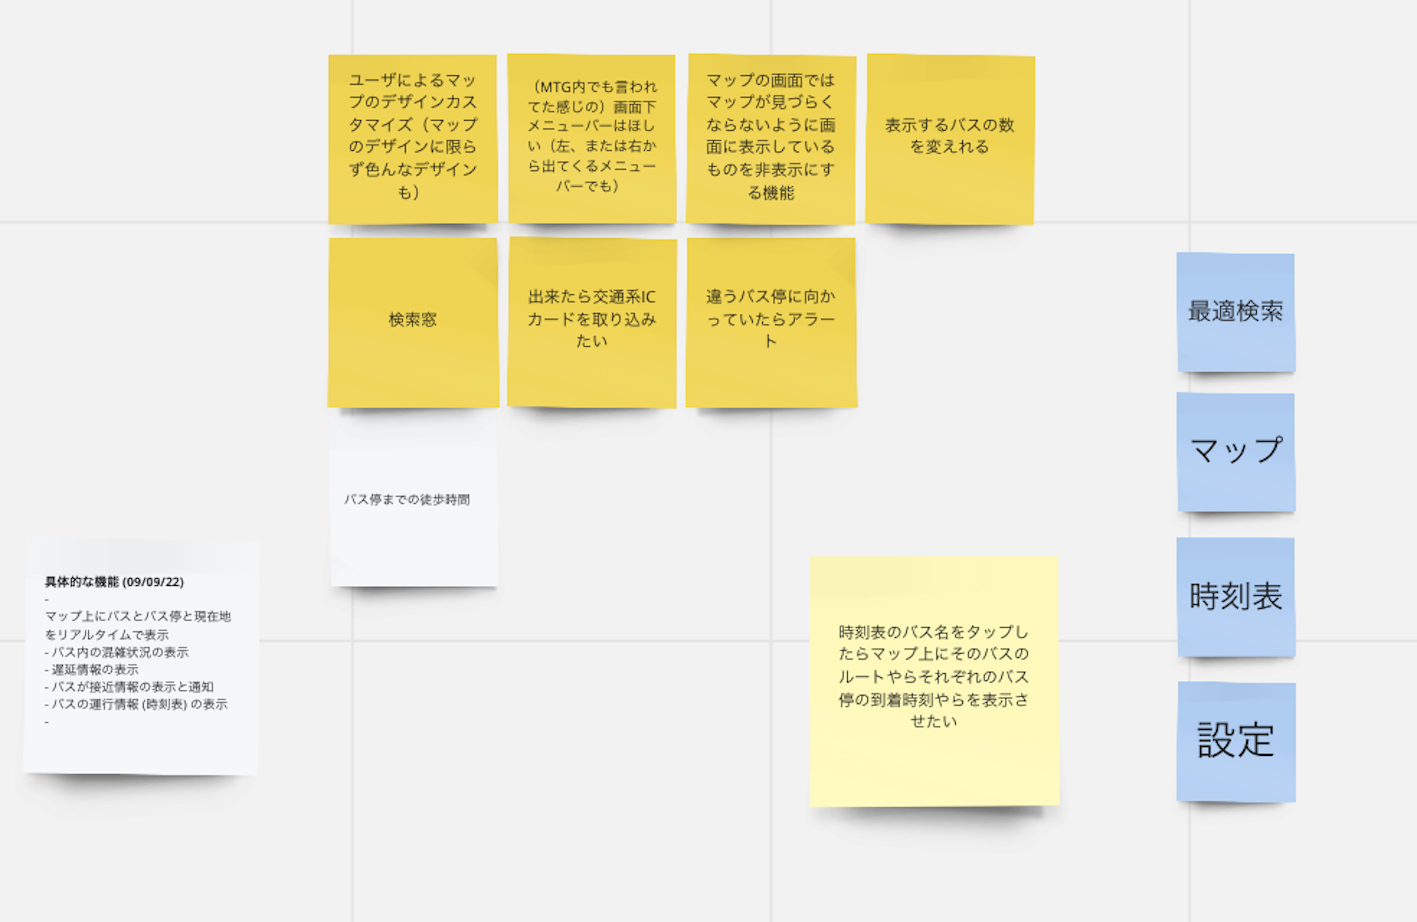
\includegraphics[width=9cm]{images/dig.png}
    \caption{アイデアの深掘り}
    \label{fig:dig}
\end{figure}
\bunseki{下村蒔里萌}

\section{アプリ名の決定}
各々が本サービスのコンセプトから考えられるサービス名を考えた.以下はその例である.
\begin{quote}
    \begin{itemize}
        \item BuLo (ブーロ) : BusとLocationの頭をとったもので,美しく (Beautiful) ,有用なユーザーインターフェースUseful (UserInterface) を持つライブ (Live) で最良のオプション (Option) である.バスロケーションシステムという意味も持つ.
        \item Loco (ロコ) :「ロケーション」と「どこ」をかけたもの.
        \item nuts (ナッツ) : No trouble with busの各単語から1文字とって組み合わせたもの.
        \item バスらく: バスをらくに使えるアプリを略したもの.横文字のアプリ名がたくさんあるが,ぱっと思い出しにくいため,名前からすぐにどんな用途かわかるものを提案した.
        \item ばすけん: バス検索を省略したもの.
    \end{itemize}
\end{quote}
上記のものでメンバー内で多数決をとった結果,BuLo (ブーロ) という名前に決定した.
BuLoはBus Locationの頭をとったものであり,
美しく (Beautiful) ,有用なユーザーインターフェースUseful (UserInterface) を持つライブ (Live) で最良のオプション (Option) であるバスロケーションシステムという意味も持つ.
\bunseki{下村蒔里萌}

\section{開発プラットフォームの決定}
まず,iOSとAndroidの2プラットフォームのネイティブアプリを並行して開発するか,クロスプラットフォームのネイティブアプリを開発するか,ということについて考えた.
本グループでは2つの理由からクロスプラットフォーム開発に決定した.
1つ目の理由は,グループの規模が小さいことである.プラットフォームを分けると,各プラットフォーム2〜3人となってしまい各人の負担が大きい.
2つ目の理由は,本グループ全体の技術力が少ないことである.
本グループには,過去に開発者としてアプリケーション開発を行ったことのある者が1人しかいない.
ほかのメンバーは経験がなく,1から学習を始めるため,学習コストが大きい.
以上の理由より,クロスプラットフォームのネイティブアプリの開発を進める形となった.
使用するフレームワークはクロスプラットフォームの代表例であるFlutter\footnote{https://flutter.dev/}となった.
\bunseki{及川寛太}

\section{メンバーの役割決定}
本グループでは4人のメンバで行っている.各メンバの役割については以下の通りである.

\subsection{プロダクトオーナー}
プロダクトオーナーはプロダクトの責任者であり,開発チームを活用して,そのプロダクトが生み出す価値を最大化する責任がある\cite{scrum}.
\begin{quote}
    \begin{itemize}
        \item 及川 寛太
    \end{itemize}
\end{quote}

\subsection{スクラムマスター}
スクラム開発を円滑に進める役割がある.
具体的に,アジャイルとスクラムの価値を維持し,ほかの人がスクラムを理解し実践するのを助ける,スクラムのミーティングをファシリテートする \cite{scrummaster}.
\begin{quote}
    \begin{itemize}
        \item 大津 武琉
    \end{itemize}
\end{quote}

\subsection{デザイナー}
問題やユーザ像の分析より,アプリのUXやUIを考え,Figma\footnote{https://www.figma.com/}でプロトタイプを作成する.
実際にプログラムを書く際に必要な,レスポンシブな数値などのデザインシステムを作成する.
\begin{quote}
    \begin{itemize}
        \item 下村 蒔里萌
    \end{itemize}
\end{quote}

\subsection{iOSアプリ}
クロスプラットフォーム開発を行うが,iOS独自の開発が必要な場合や問題が発生した場合に,優先的に対応にあたる.
\begin{quote}
    \begin{itemize}
        \item 及川 寛太
        \item 下村 蒔里萌
    \end{itemize}
\end{quote}

\subsection{Androidアプリ}
クロスプラットフォーム開発を行うが,Android独自の開発が必要な場合や問題が発生した場合に,優先的に対応にあたる.
\begin{quote}
    \begin{itemize}
        \item 大津 武琉
        \item 稲田敬介
    \end{itemize}
\end{quote}

\subsection{サーバサイドエンジニア}
バスの運行に関わるデータの収集・記録・管理を行う.また,クライアント側が必要とする情報を素早く提供するシステムを開発する.
\begin{quote}
    \begin{itemize}
        \item 及川 寛太
        \item 大津 武琉
    \end{itemize}
\end{quote}
\bunseki{大津武琉}

\section{Git・GitHubの習得}
チーム開発を進める中で必要不可欠であるバージョン管理アプリのGitHub\footnote{https://github.com/}の勉強会を行なった.メンバーの過半数がGitHubを触ったことがなかったため,使用経験がある人から基本的な使用方法を教えてもらい,実際にGit\footnote{https://git-scm.com/}の機能であるClone,Commit,Push,Fetch,Merge,Pullを行なってGitHubについて学んだ.
\bunseki{稲田敬介}

\section{プロトタイプの作成}
\subsection{プロトタイプver.1}
アプリのプロトタイプをFigma\footnote{https://www.figma.com/}を用いて作成した (図\ref{fig:prototype_v1}) .
左から1枚目の画面は自分の現在地を表示させている.
2〜4枚目は目的地を入力する画面となっている.
5〜6枚目は現在地から2〜3枚目で入力した場所までのバスを表示させる.
7枚目では5〜6枚目で選択したバスと自分との位置関係をグラフと地図で表示させる.

\begin{figure}[H]
    \centering
    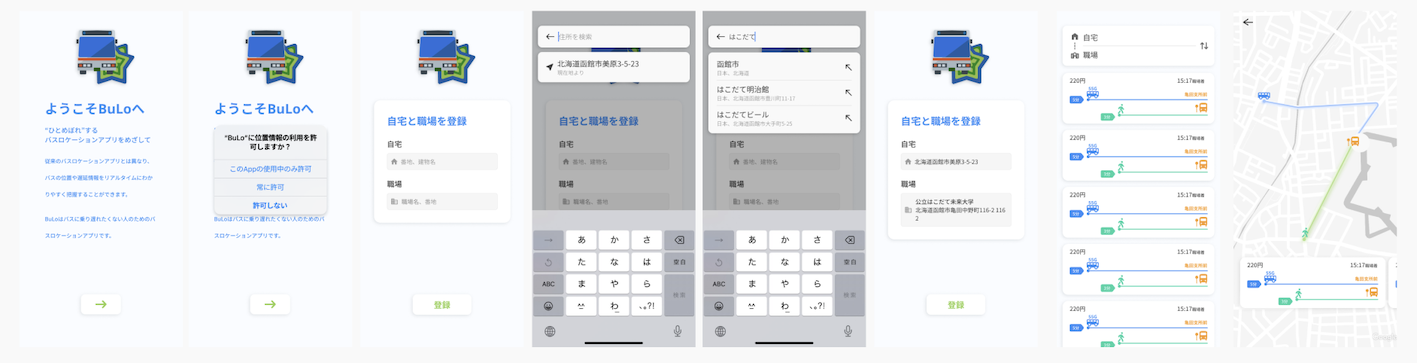
\includegraphics[width=12cm]{images/prototype_v2.png}
    \caption{プロトタイプver.1}
    \label{fig:prototype_v1}
\end{figure}

\subsection{フィードバック}
実際にプロジェクトメンバにFigma\footnote{https://www.figma.com/}で作成した図\ref{fig:prototype_v1}のプロトタイプを使用してもらった.
その際たくさんの質問,指摘,意見をいただいた.一番右の画面に対して,「下のバスと人との位置関係のグラフはいるのか?」,
「現在動いているバスの位置情報と自分の位置情報が分かれば大体どれくらいにバス停にいけばいいのかわかるのでは?」という意見をいただいた.
それらの意見に対し,ターゲットユーザを絞ることとした.

実際に得たフィードバックから,ターゲットユーザが定まっておらず,このアプリは何のため,誰のためのアプリなのかがわからないことに気がついた.
そこでチームでもう一度ターゲットユーザについて話し合い以下のように確立させた.

\begin{quote}
    \begin{itemize}
        \item 通勤通学にバスを使っていて,バスの乗降地点が毎回同じ
        \item バスに乗り遅れたくない
        \item バス停で待ちたくない
        \item 10代後半から20代前半
    \end{itemize}
\end{quote}

\subsection{プロトタイプver.2}
確立させたターゲットユーザに合う機能のみを実装するとしたため,合わせてプロトタイプを改善した.

図\ref{fig:prototype_v1}のプロトタイプではユーザが毎回移動先・移動元を検索していたが,
最初に登録をすることで,検索を毎回行う工程を省いた.通勤通学など,使用するバスが決まっているというユーザ像には,
地点の検索は無駄な工程であった.

アプリ全体のデザインとしては,色やアイコンを改善した.
具体的には,Time-Distace Viewのアイコンとその色を変更した.以前は人のアイコンが走っている人間のアイコンであり,
赤色を使用していたため,焦りを与えていた.そのため,色を改善し,さらに同レベルの情報の色のコントラストを揃えた.
また,Flutter\footnote{https://flutter.dev/}で開発をするにおいて,アイコンをMaterial Designに統一した.

Time-Distance Viewについて,どの駅を使用するのか,何円かかるか,何時に到着するかなどの,ユーザが必要最低限と感じる情報を追加した.
さらに,ウィジェット全体のサイズやレイアウトを改善した.

最後に,アプリを開いた時にランディング画面を設けることで,アプリ全体の概要や印象をユーザがわかりやすくなるよう改善した.

\begin{figure}[H]
    \centering
    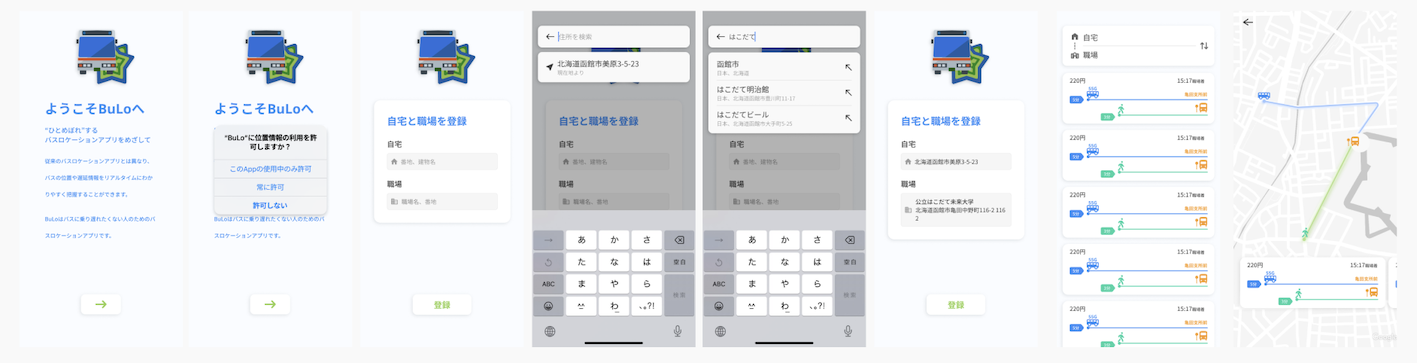
\includegraphics[width=12cm]{images/prototype_v3.png}
    \caption{プロトタイプver.2}
    \label{fig:prototype_v2}
\end{figure}

\subsection{フィードバック}
後述する中間発表や会やUCDワークショップにて,プロトタイプver.2を使用してもらった.
その際たくさんの質問,指摘,意見をいただいた.
図\ref{fig:prototype_v1}の左から7,8枚目の画面に対して,「グラフの右端がバス停であることがわかりづらい」,
左から1〜3枚目の画面に対して,「登録ボタンの視認性が悪い」という意見をいただいた.

\subsection{プロトタイプver.3}
図\ref{fig:prototype_v3}の左から1〜3枚目の画面は初期画面である.
4〜6枚目は目的地を入力する画面となっている.
7枚目は現在地から4〜3枚目で入力した場所までのバスを表示させる.
8枚目では4〜6枚目で選択したバスと自分との位置関係をグラフと地図で表示させる.
図\ref{fig:prototype_v2}へのフィードバックをもとに,バスと現在地の時間的なグラフを改善した.
また,図\ref{fig:prototype_v3}の左から4〜6枚目の画面,すなわち目的地入力画面では,登録ボタンの視認性を向上させた.

\begin{figure}[H]
    \centering
    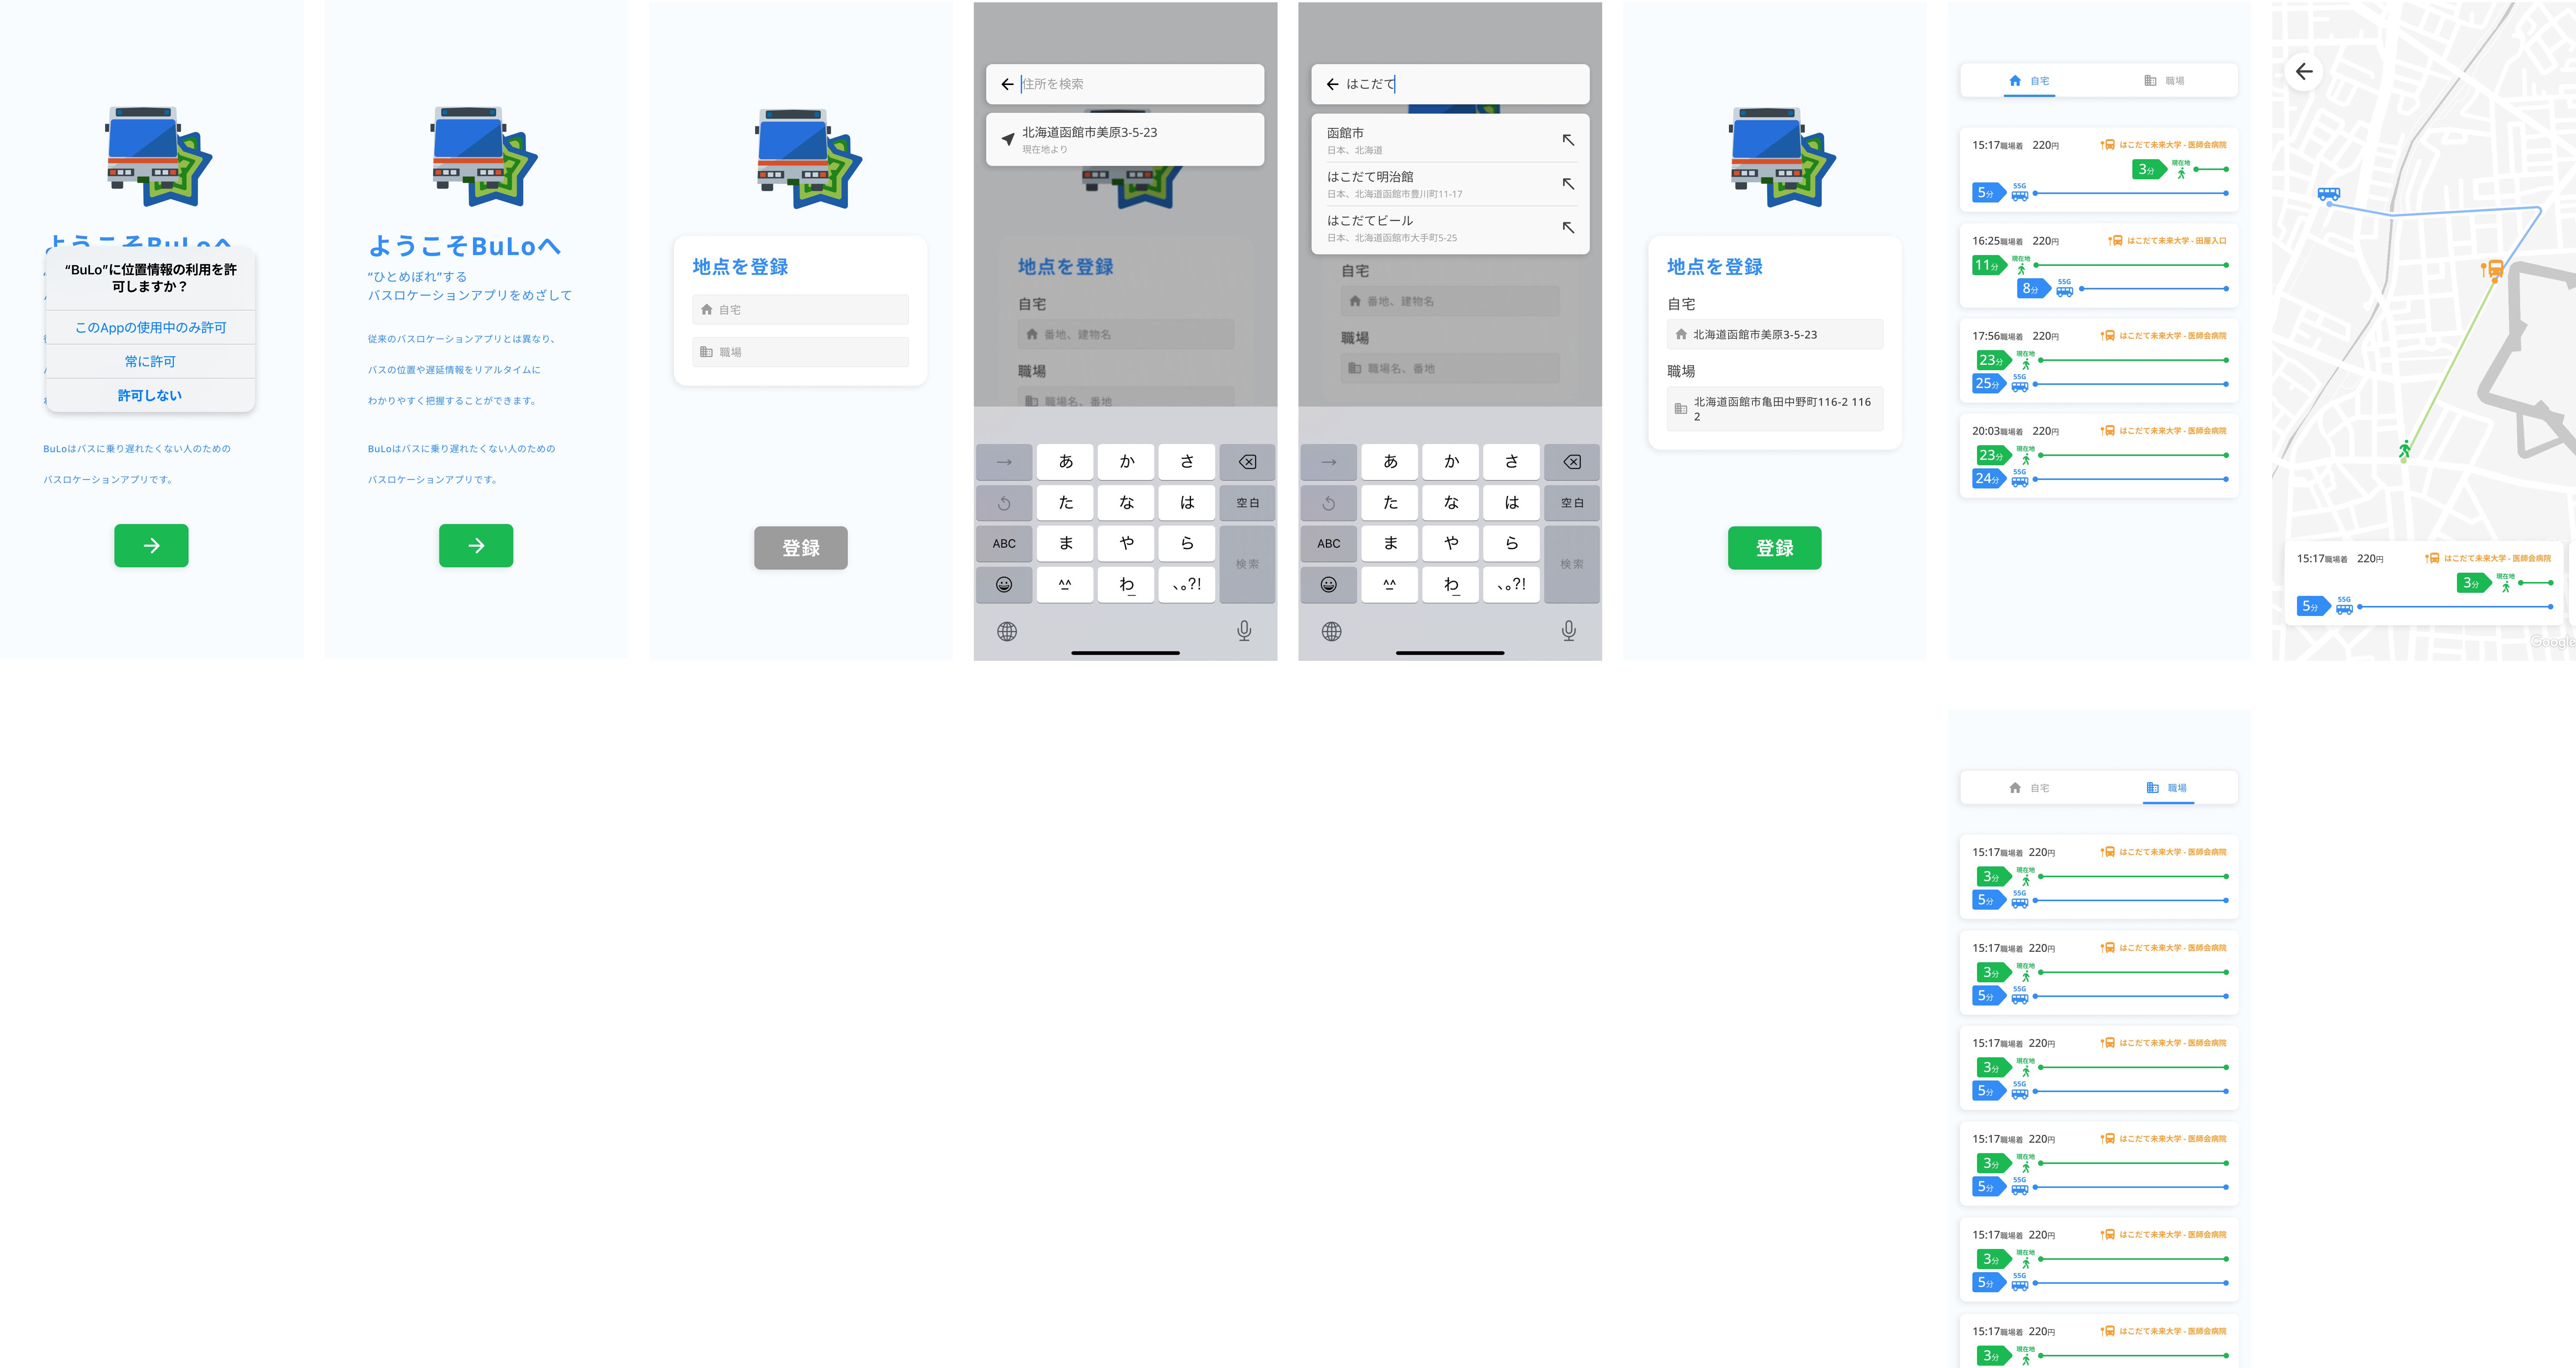
\includegraphics[width=12cm]{images/prototype_v4.png}
    \caption{プロトタイプver.3}
    \label{fig:prototype_v3}
\end{figure}
\bunseki{下村蒔里萌}

\section{リスク分析}
プロジェクトを行ううえでリスクは必ず存在する.
リスクマネジメント\cite{risk}はそのリスクに対してどのように対策するのかを考える.まず初めにプロジェクトメンバーを3グループに分け,それぞれのチームでメンバーが持ち寄った起こりそうなリスクをまとめた.
その後それぞれのリスクに対して,そのリスクが被る被害,発生確率,影響度,脅威,対策を考えた.脅威については発生確率,影響度を掛け合わせたものであり,脅威の値が大きいほど対策するべき優先度が高いものとなる.
まとめたリスクの中でも,特に脅威の値が高いリスクを以下に示す.

\begin{table}[]
    \begin{tabular}{lll}
    リスク       & 被害             & 対策                                                                                                                                                                             \\ \hline \hline
    技術・知識不足   & 作業の停滞 & \begin{tabular}[c]{@{}l@{}}回避:普段から会話をし、様子を知っておく\\ 軽減:役割分担に余裕を持つ、\\一人しか把握していないタスクを作らない、\\ できる人に聞く(他のメンバーやTA、教授など)、\\猛勉強する\\ 転嫁:タスクを再分配する、\\再分配してもいいように余裕を持つ\end{tabular} \\\hline
    コンピュータの破損 & データ紛失          & \begin{tabular}[c]{@{}l@{}}回避:クラウド等に定期的にバックアップを取る、\\PCの使い方に気を付ける\\ 軽減:バックアップ、データのバックアップ、\\ 転嫁:メーカー保証、保険をかける\end{tabular}                                                         \\\hline
    開発環境の不具合  & 開発できない         & \begin{tabular}[c]{@{}l@{}}軽減:開発環境構築をドキュメント化しておく\\(→再構築がしやすい)、\\ みんな同じ環境が作れる、他の開発環境を使用する\end{tabular}                                                                           \\\hline
    やる気不足     & 作業の停滞          & \begin{tabular}[c]{@{}l@{}}回避:人の目があるようなところで作業する\\ 軽減: モチベアップしそうな目標を立てる\\ 転嫁: 気分転換に遊ぶ\end{tabular}                                                            \\\hline
    データ消失     & データ紛失          & \begin{tabular}[c]{@{}l@{}}回避:定期的にバックアップを取る、\\共有ファイルを作る                          \end{tabular}                                                                                                                           
    \end{tabular}
\end{table}
\clearpage

脅威に対して行うことができる対策には回避,軽減,転嫁,受容の4つがある.
例えば一番上の「プログラム等の技術不足」に関しては,被害が「作業の停滞,メンバへの迷惑」ということになり,これに対して取ることができるのは役割分担に余裕を持つ,出来る人に聞く等の「軽減」対策,タスクを再分配する,再分配してもいいように余裕を持つ等の「転嫁」対策ということとなる.
このようにしてリスクを分析し,それに関して対策を事前に決めておくことで,迅速かつ最適な行動を被害発生時にとることができる.
\bunseki{稲田敬介}

\section{函館バス株式会社への訪問}
函館バス株式会社は,バス運行に関するデータを公開していないため,
本グループが開発しているアプリの紹介と,データを使用させていただくために,6月16日 (金) に本グループメンバーと担当教員で函館バス株式会社に訪問した.
そこで函館バス株式会社の方から「新しい観点からの機能で良い」というお言葉をいただき,データの使用の許可をいただいた.

\begin{figure}[H]
    \centering
    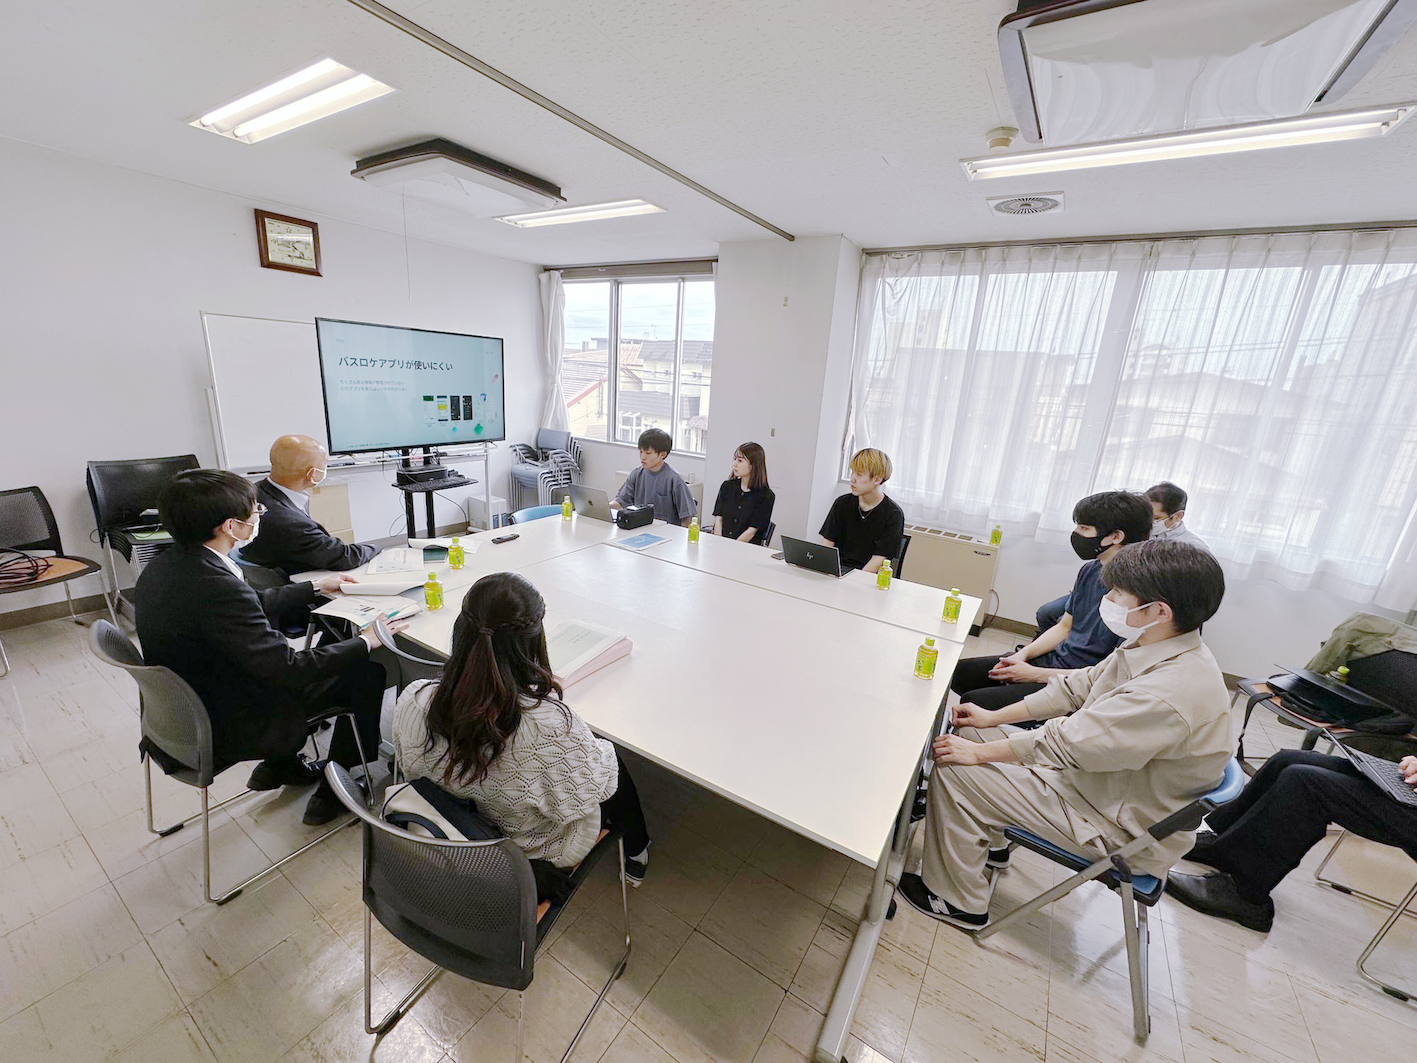
\includegraphics[width=9cm]{images/hakodate_bus.png}
    \caption{函館バス株式会社訪問時の様子}
    \label{fig:hakodate_bus}
\end{figure}
\bunseki{大津武琉}

\section{中間発表}
\subsection{中間発表資料の作成}
7月7日 (金) に行われる中間発表会に向けてスライド,メインポスター (図\ref{fig:interim_poster}) ,サブポスター (図\ref{fig:interim_poster_bulo}) を作成した.これらの資料に関して教員に繰り返しレビューをしていただき,より伝わりやすいものへと改良を重ねた.

\begin{figure}[H]
    \centering
    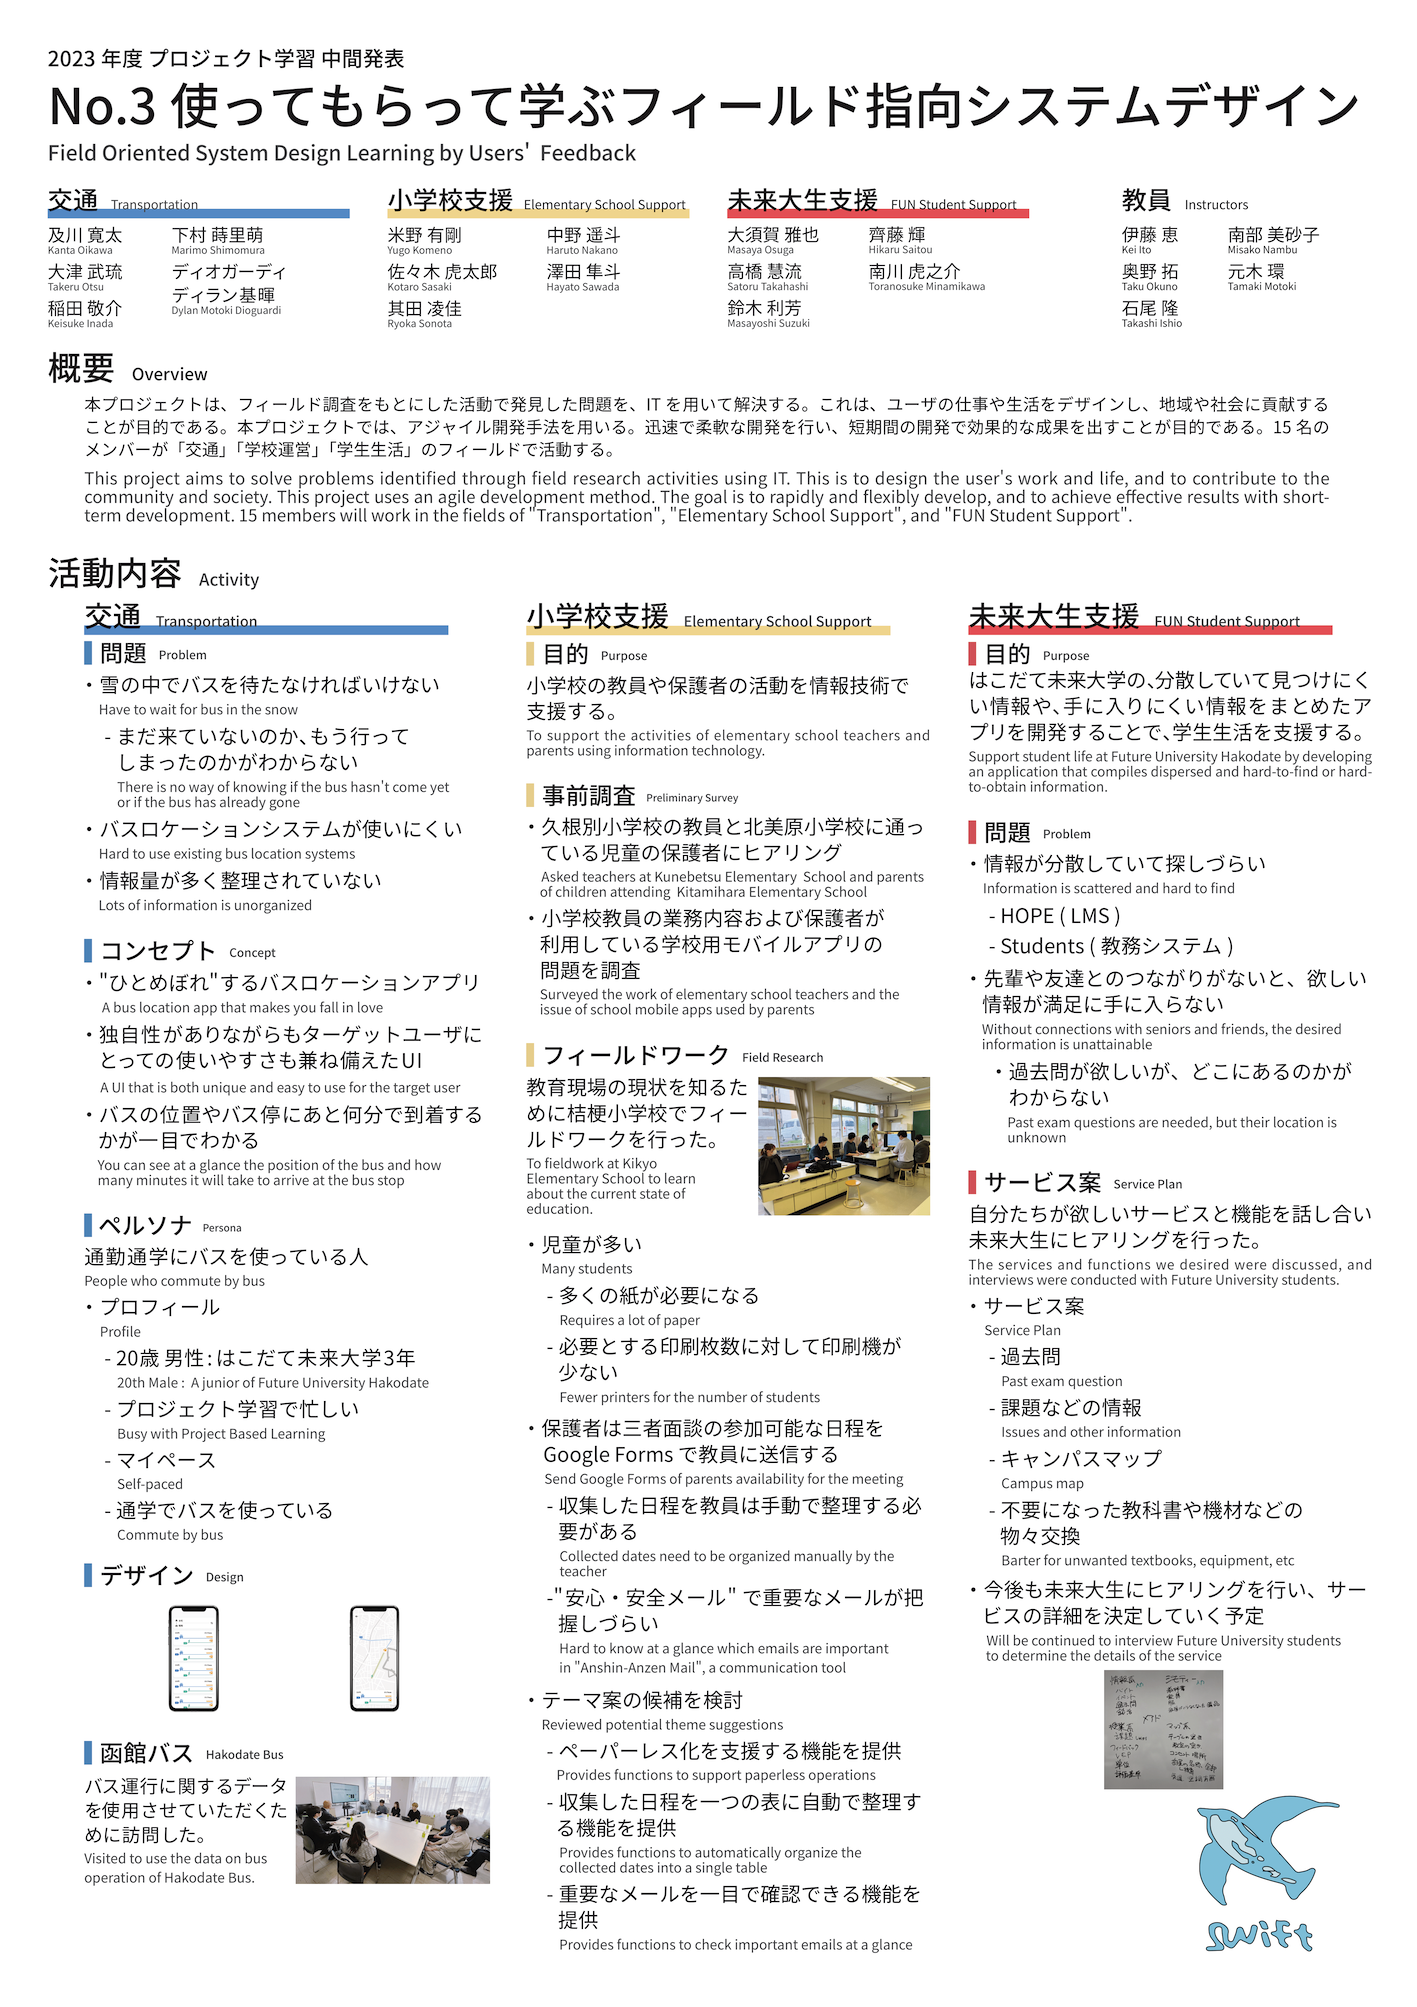
\includegraphics[width=9cm]{images/interim_poster.png}
    \caption{中間発表会メインポスター}
    \label{fig:interim_poster}
\end{figure}

\begin{figure}[H]
    \centering
    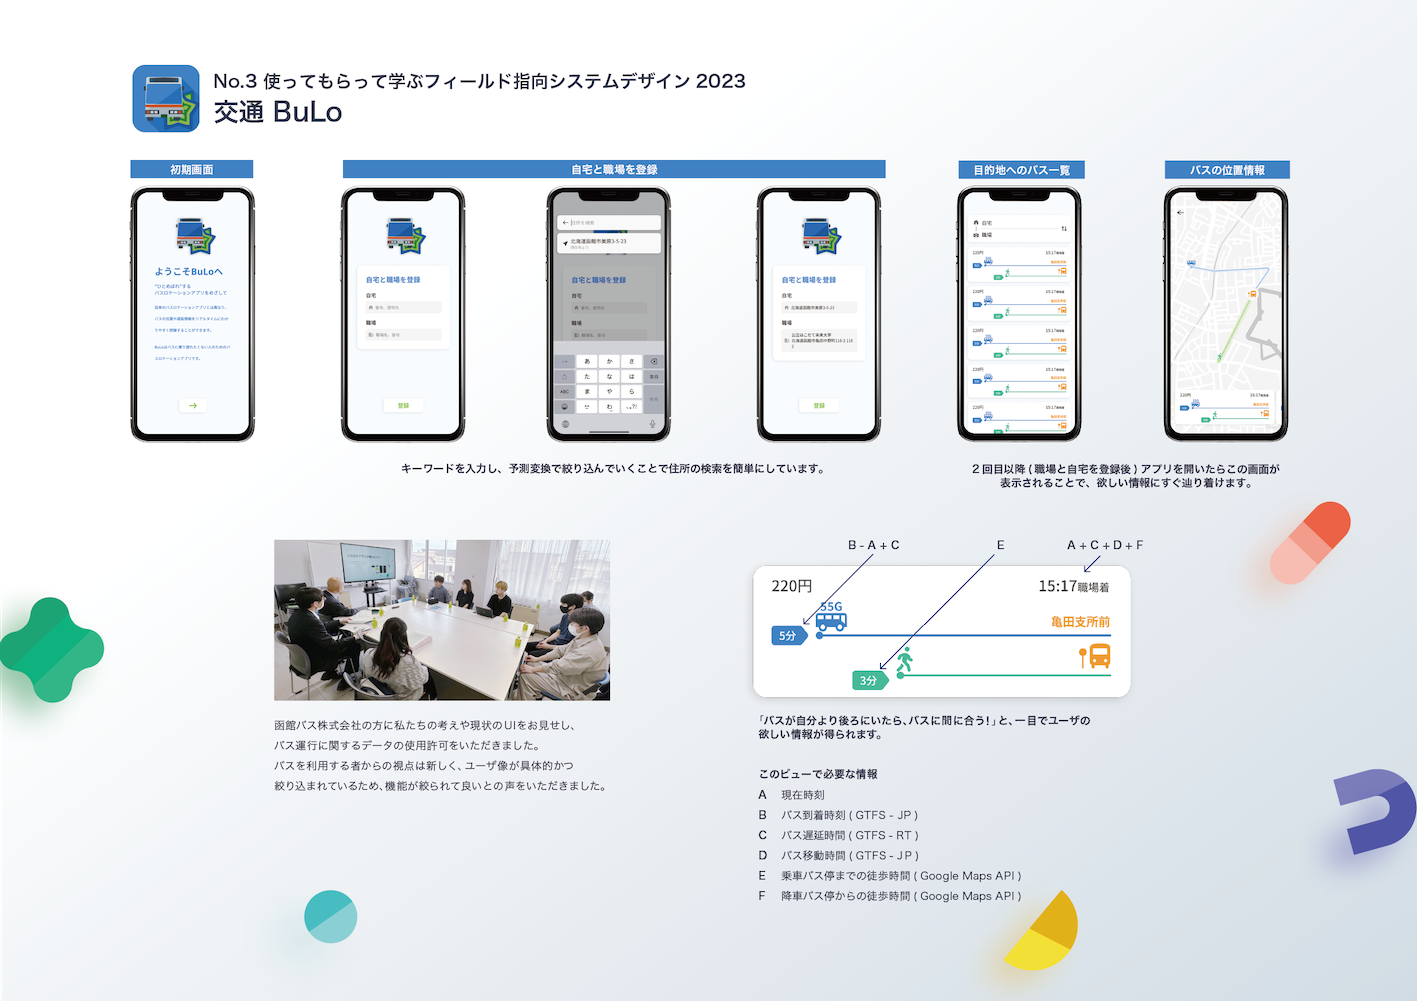
\includegraphics[width=9cm]{images/interim_poster_bulo.png}
    \caption{中間発表会サブポスター}
    \label{fig:interim_poster_bulo}
\end{figure}

\subsection{中間発表会}
7月7日 (金) に発表会は行われた.そこで様々な質問や意見をいただいた.「首都圏と函館で同じ状況を想定していいのか?」「独自性を掲げているがUIについての独自性のみで機能についての独自性がみられない」という指摘をいただいた.これらの意見は,ターゲットユーザを絞り,合わせて実装する機能を絞った結果であると考えているため,次期バージョンにていただいた指摘をもとに改善を行う.

\begin{figure}[H]
    \centering
    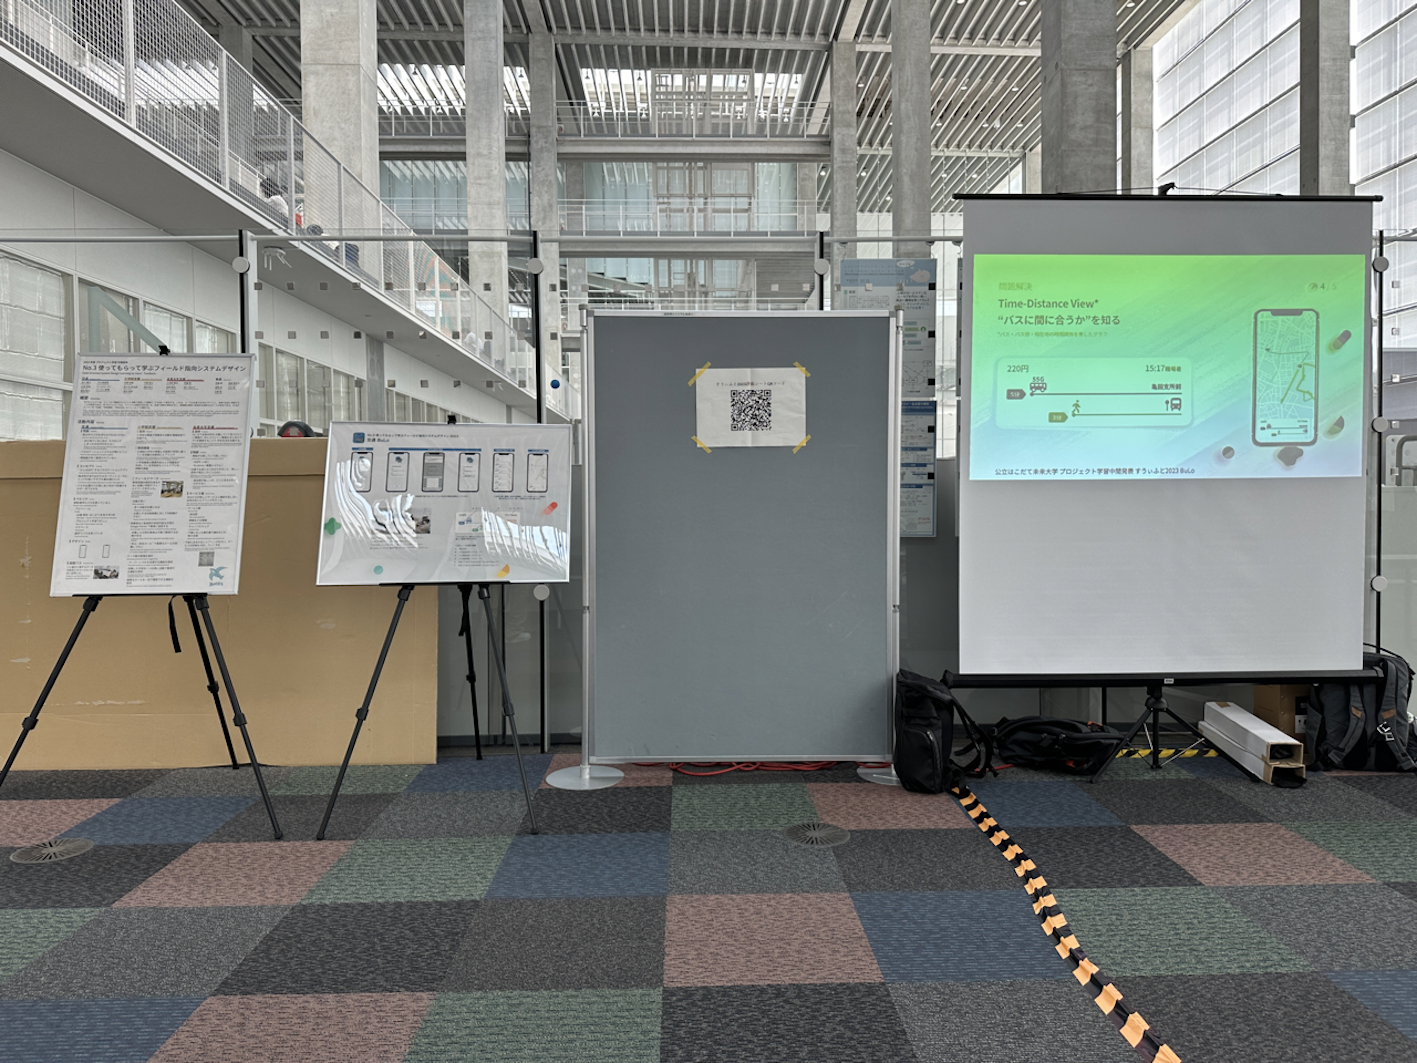
\includegraphics[width=12cm]{images/mid_presentation.png}
    \caption{中間発表会の様子}
    \label{fig:mid_presentation}
\end{figure}
\bunseki{下村蒔里萌}

\section{開発}
\subsection{アジャイル開発}
\subsubsection{スクラム}
\subsubsection{デザインシステム}
\subsection{使用したツール}
\subsubsection{Discord}
\subsubsection{Figma}
\subsubsection{GitHub Projects}
\subsubsection{Notion}

\section{UCDワークショップ}
9月17日 (日) ,9月18日 (月) に希望するメンバでUCDワークショップに参加した.UCDワークショップとは,enPiTという高度IT人材の育成を目指している
取り組みの一つである.このワークショップでは,大阪芸術大学の木塚あゆみ先生をお招きして人間中心のデザイン,ユーザ・センタード・
デザイン (それぞれの頭文字を取ってUCD) の考え方とその設計方法を,短期集中の講義と演習を通して学んだ.演習では,20年後の未来で使いたい製品・
サービスを考え,シナリオ形式で発表した.グループの他のメンバとの話の噛み合いよく進行するためビジュアルシンキングを用いてアイデアを共有したり,
ヒューマン・センタード・デザイン (HCD) を意識して避けたりするなど,アイデアを評価しながら洗練されたものにしていくまでの手順を実践した.
\bunseki{稲田敬介}

\section{アカデミックリンク}
11月3日 (金) にはこだて高等教育機関合同研究発表会,通称HADKOTEアカデミックリンクに参加した.HAKODATEアカデミックリンクは,函館市内にある8つの大学,
短大,高専で日々行われる研究を市民・地元企業の方々にわかりやすく披露する場として提供されたもので,今年度のHAKODATEアカデミックリンク2023は
キャンパス・コンソーシアム函館加盟校8校の学生をはじめ,函館市内の高校生や他地域の大学生などが函館アリーナを会場に4年ぶりに対面で開催されたものであった.
\bunseki{稲田敬介}

\section{成果発表会}
\subsection{成果発表会資料作成}
12月8日 (金) の成果発表会に使用するプロジェクト全体用のメインポスター,グループ発表用のグループポスター,発表スライドを作成した.これらの資料は教員に
随時レビューを求め,わかりやすい資料になるよう改良を重ねた.

\begin{figure}[H]
    \centering
    \includegraphics[width=9cm]{images/final_main_poster.png}
    \caption{成果発表会メインポスター}
    \label{fig:final_main_poster}
\end{figure}

\begin{figure}[H]
    \centering
    \includegraphics[width=9cm]{images/poster.png}
    \caption{成果発表会サブポスター}
    \label{fig:poster}
\end{figure}

\bunseki{稲田敬介}

\subsection{概要}
12月8日 (金) に成果発表会が行われ,そこでは未来大内外問わず,様々な方々からな意見や質問をいただくことができた.説明資料としてブースに配置していたポスター,デモ機,ま
た,発表とそれに用いたスライド等を通して,「TDViewにリスト表示されている分数を表すゲージの長さは,相対的に決めるのでは分かりづらいのではないか?」といったUIに関する意見や
,「データの管理方法や精度はどのようになっているのか」など,データの取扱に関する質問をいただくことができた.またその一方で,「このアプリがリリースされたら使いたい」といったニーズが存
在することを確認できた.
\bunseki{稲田敬介}

\section{enPiT BizSysD 北海道・東北合同発表会}
2月9日 (土) にWebとZoom上にて行われた,enPiT BizSysD 北海道・東北合同発表会に参加した.この発表会はいくつかの他大学と合同で行われ,全8チームのエントリーとなった.
発表資料としては,前日に行われた成果発表会にて使用した資料をそのまま用いた.発表を通して教員・学生等様々な方々から評価をしていただくことができ,アイデア部門の最優秀賞,
全体を通しての最優秀賞をいただくことができた.また,他大学の利用する技術,アイデア等を拝見できる貴重な機会として,充実した発表会となった.
\bunseki{稲田敬介}

\section{最終報告書執筆}
最終報告書の執筆には成果発表会後に取り組み始めた.まず全体的な報告書の構造を作成し,その後それぞれの章に対して文章を担当するメンバを振り分けた.構造に関しては前年度に作成された最終報告書
を参考にしつつも,不必要に感じるものを削ぎ落とし,章の順序を見直すなどして再構築した.グループ内の仮完成日を1月12日 (金) と定め,メンバはそれぞれの章でtexファイルを作成し,割り当てられた章を執筆することとした.
プロジェクト報告書の担当箇所に関しては稲田が記述し,他メンバからのレビューを経て全体に提出した.
\bunseki{稲田敬介}
